\documentclass[12pt]{article}
\usepackage[english]{babel}
\usepackage[utf8x]{inputenc}
\usepackage[T1]{fontenc}
\usepackage{scribe}
\usepackage{listings}
\usepackage{hyperref}
\usepackage{tikz}
\usepackage{mdframed}
\usepackage{float}
\usepackage{array}
\usepackage{algorithmic}
\usepackage{algorithm}

\usepackage{pythonhighlight}


\newcommand{\vect}[1]{\mathbf{#1}}
\newcommand{\rdbracket}[1]{\left( #1 \right)}
\newcommand{\sqbracket}[1]{\left[ #1 \right]}
\newcommand{\lgbracket}[1]{\left\{ #1 \right \}}
\newcommand{\iid}[0]{ \overset{\text{iid}}{\sim}}
\newcommand{\myVec}[1]{\mathbf{#1}}
\newcommand{\highlight}[1]{\textcolor{blue}{\textit{#1}}}
\newcommand{\confusion}[1]{\textcolor{red}{\textit{#1}}}




\Scribe{Yuhao Wu}
\LectureDate{DATE: 2020-07-18}

\lstset{style=mystyle}

\begin{document}
	\MakeScribeTop
GAN(Generative Adversarial Network) is first raised by Ian Goodfellow in his paper "Generative Adversarial Network" \cite{goodfellow2014generative}. Of course, from its name, we know that GAN is to generate something. One of its greatest application is in "Face Generation". In the end of 2019, NVIDIA published their "StyleGAN2" \cite{karras2020analyzing}(\highlight{code available}), which is to produce fake face picture with resolution $1024 \times 1024$. GAN is also highly recognized by Yann LeCun. He said "Adversarial training is the coolest thing since sliced bread".


\section{Basic Structure}
For GAN, it should have one "Generator" and one "Discriminator", the basic structure is shown in figure \ref{fig:basicStructure} below.
\begin{figure}[H]
    \centering
    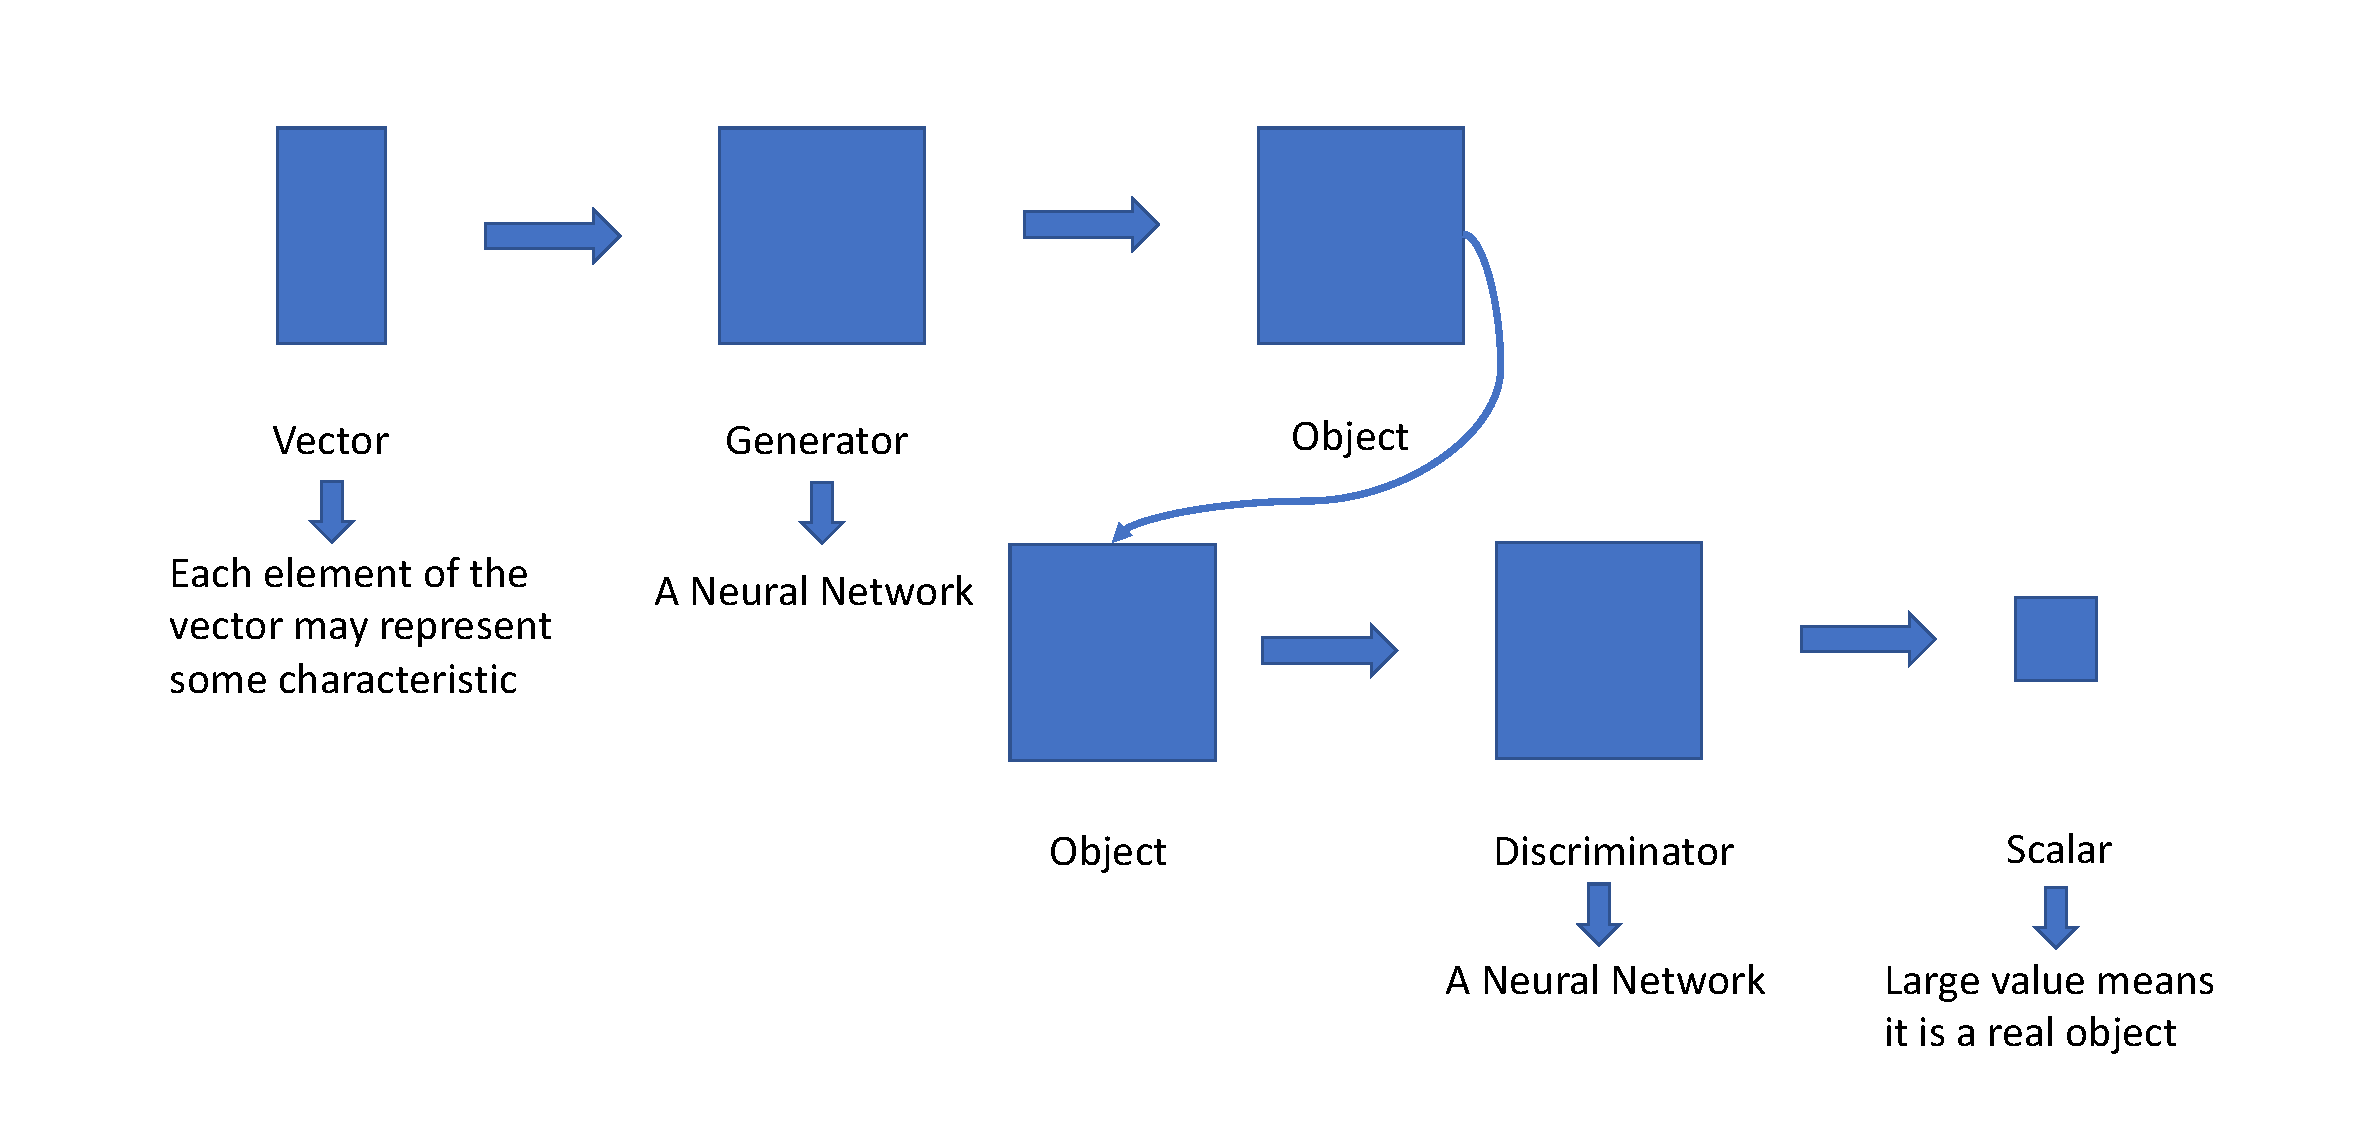
\includegraphics[width = \textwidth]{basicStructure.pdf}
    \caption{Basic structure of GAN}
    \label{fig:basicStructure}
\end{figure}

For the object, it can be one picture, or a 3D mesh, or maybe a sentence. According to what you want, you may need to do some change on the output layer of "Generator". If you want a sentence, you may need a RNN; if you want a picture, you may add one deconvolution.

For the vector, we say each element of the vector may represent some characteristic. We assume that our output is a manifold in a higher dimension. So, the vector is the best for data with the same dimension. \highlight{But how do we know how many dimension we need. We have no idea. Looks like it is a hyper-parameter.} 

\section{Theoretical Result of GAN}
\subsection{Value Function}
\begin{itemize}
	\item $G(z; \theta_g)$ is a differentiable function represented by a multilayer perceptron with parameters $\theta_g$. Its input is one latent space variable $z$.
	\item $D(x; \theta_d)$ is a differentiable function represented by a multilayer perceptron with parameters $\theta_d$. 
\end{itemize}
What we want to optimize is the following value function:
\begin{equation}
\min_G \max_D V(D, G) = \min_G \max_D\ \E_{x \sim p_{data}(x)}[\log(D(x))] + \E_{z \sim p_z(z)} [\log(1 −D(G(z)))] .
\end{equation}
Since it is binary classification under this "Discriminator", we have the following cross entropy:
\begin{equation}
	H((x,y), D) = - \Big[ y \log(D(x)) + (1 - y) \log(1 - D(x_1)) \Big]
\end{equation}
For infinite data point we have:
\begin{equation}
	H((x,y)_{i = 0}^{\infty}, D) = - \sum_{i = 0}^{\infty} \Big[ y \log(D(x)) + (1 - y) \log(1 - D(x_1)) \Big].
\end{equation}
For each $x_i$, it is either from the true data, which should satisfy $x \sim P_{data}(x)$; or it is from the "Generator", which should satisfy $x = G(z), z \sim P_Z(z)$. We separate the datas apart. If it is from the real data, it would zero out the latter part of Equation(3); if it is from the "Generator", it would zero out the first part of Equation(3). When we are doing training, we would provide half of the data from "Generator", half from real data. So, the $P(y = 1) = P(y = 0) = \dfrac{1}{2}$. Thus, we have:
\begin{equation}
	H((x,y)_{i = 0}^{\infty}, D) = - \dfrac{1}{2} \Big[ \E_{x \sim p_{data}(x)}[\log(D(x))] + \E_{z \sim p_z(z)} [\log(1 −D(G(z)))] \Big].
\end{equation}
\highlight{The above statement comes from Ian's 2016 tutorial \cite{goodfellow2016nips} section 3.2 "Cost Function". If you have time, could you please check if I understand them right. }


It needs to minimize the maximum value of $V(D, G)$. Intuitively speaking, it is really easy to understand: we would train the "Discriminator" first, which is trying to make the "Discriminator" give real images scores as high as possible. Then, we need to train the "Generator", which is trying to make the "Generator" produce fake images to confuse the "Discriminator" so that "Discriminator" would give real image low scores. 

\subsection{Convergence of the Algorithm}
The "Generator" generates data $G(z)$ when $z \sim P_z$. We can say that the generator $G$ implicitly defines a probability distribution $p_g$. According to \cite{goodfellow2014generative}, Section 4, Ian has proved that Algorithm1 would converge $p_g$ to a good estimator of $p_{data}$, if given enough capacity and training time. 



\begin{figure}[h]
\begin{tabular}{m{3cm}m{3cm}m{3cm}m{0.1cm}m{3cm}}
    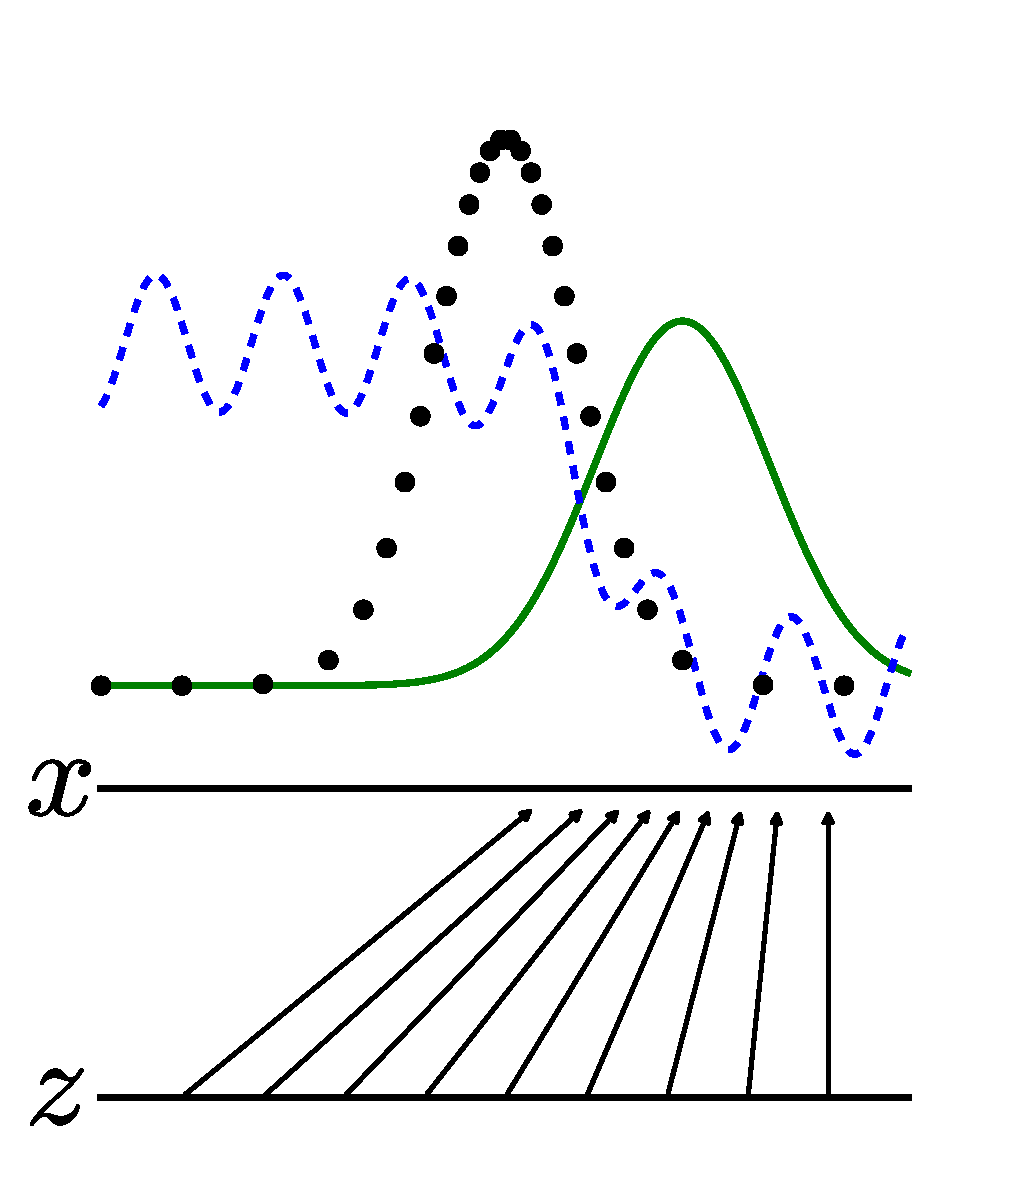
\includegraphics[width=3cm, height=4cm]{fig1.pdf} 
    &  
    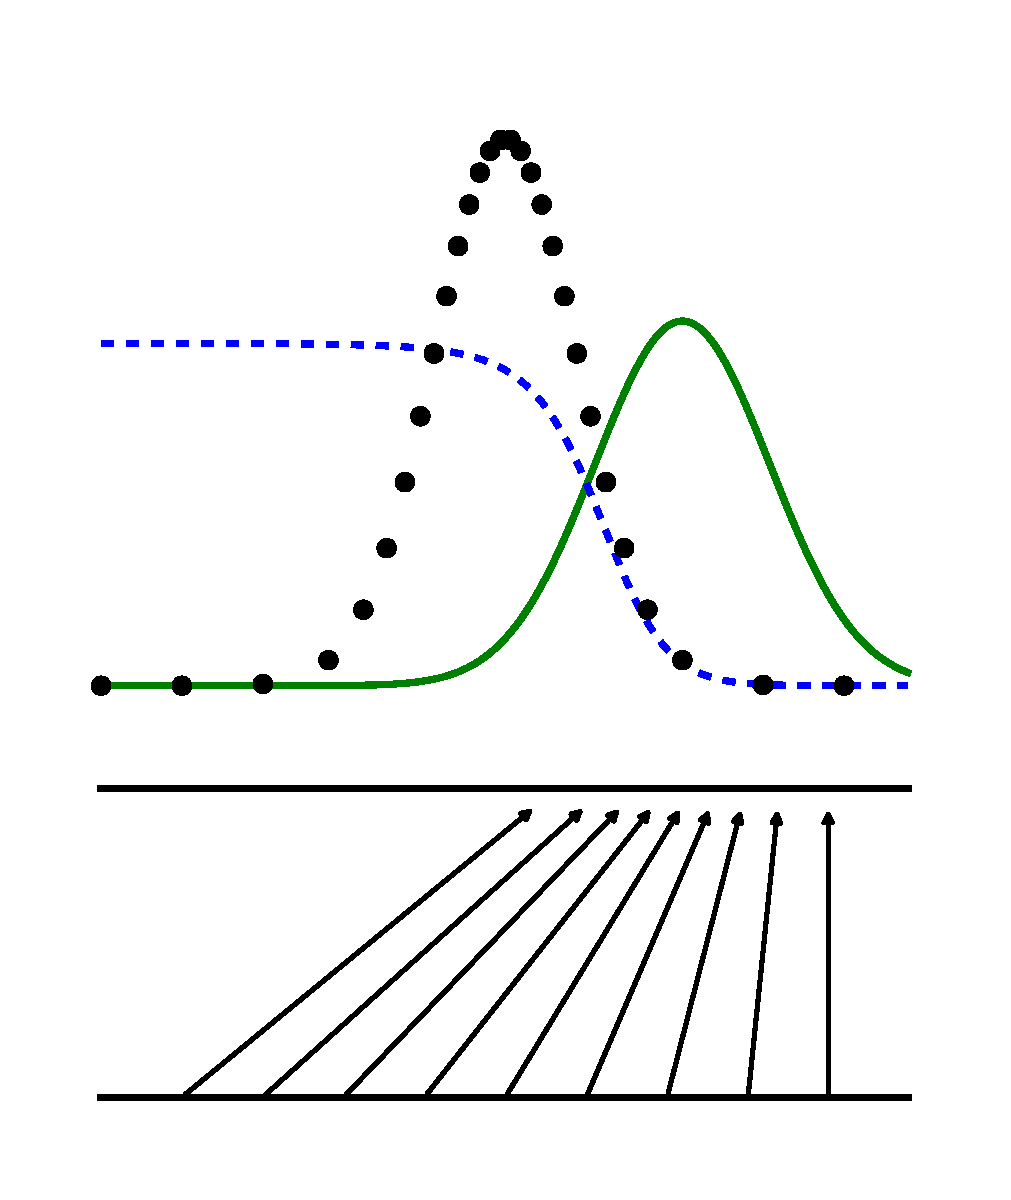
\includegraphics[width=3cm, height=4cm]{fig2.pdf}
    & 
    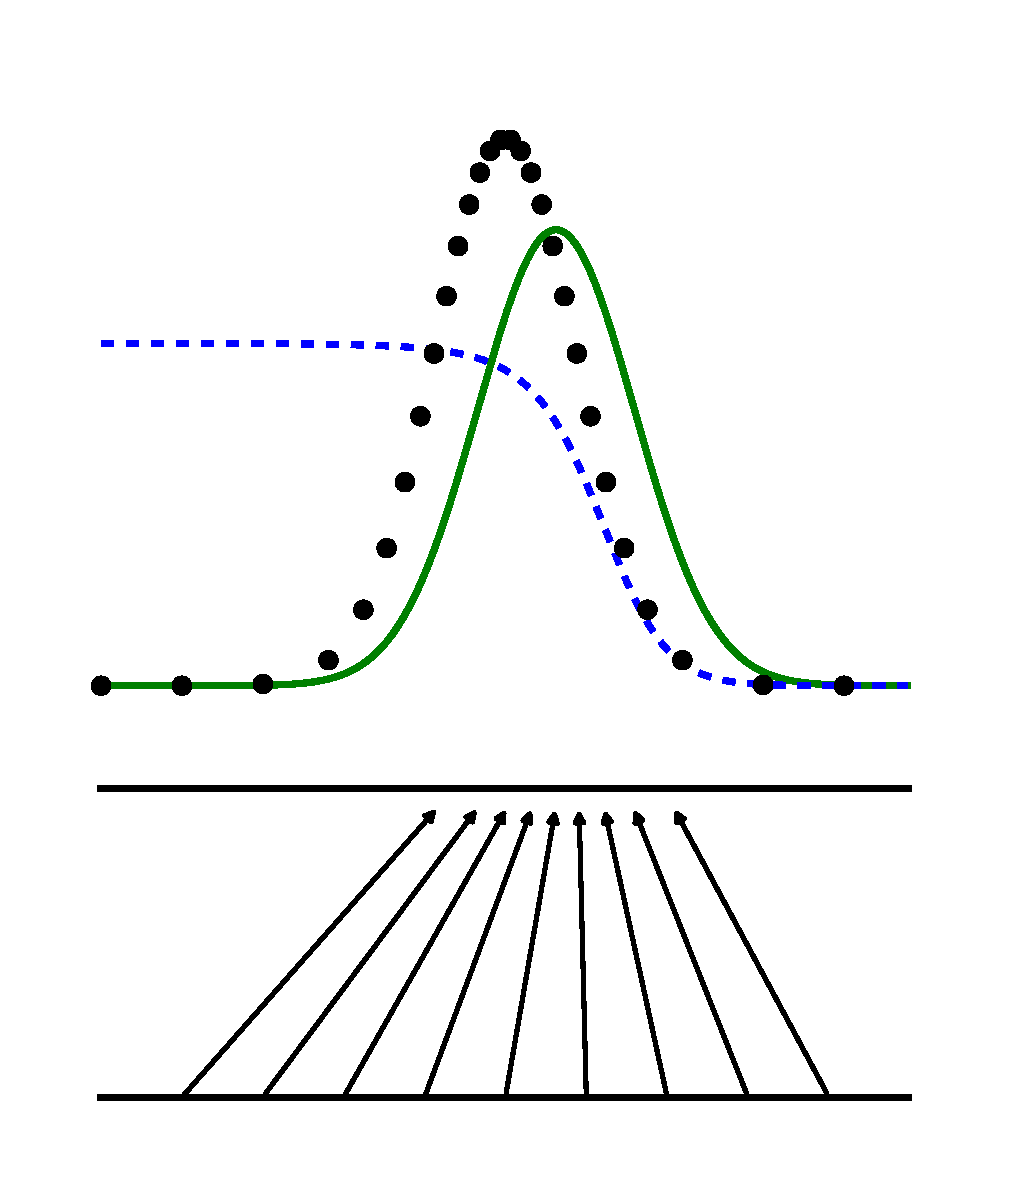
\includegraphics[width=3cm, height=4cm]{fig3.pdf}
    &
    \dots
    &
    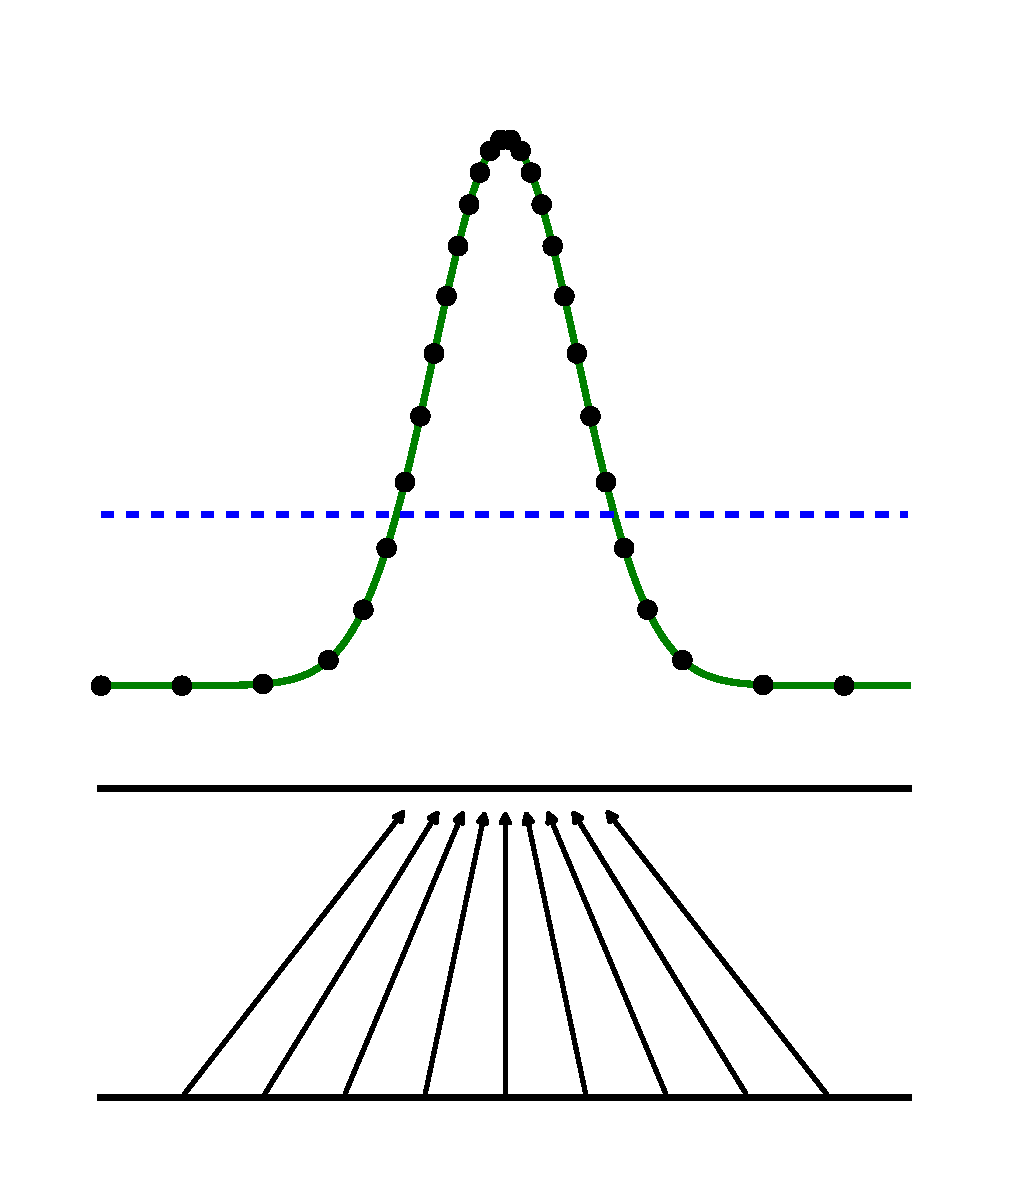
\includegraphics[width=3cm, height=4cm]{fig4.pdf}
    \\
    \centering (a)
    & 
    \centering (b) 
    & 
    \centering (c) 
    &  
    & 
    \centering (d)
\end{tabular}

\caption{\small
Generative adversarial nets are trained by simultaneously updating the \textbf{d}iscriminative 
distribution ($D$, blue, dashed line) so that it discriminates between samples from
the data generating distribution (black, dotted line)
$p_{\bm{x}}$ 
from those of the \textbf{g}enerative distribution $p_g$ (G) (green, solid line).
The lower horizontal line is the domain from which $\bm{z}$ is sampled, in this case uniformly.
The horizontal line above is part of the domain of $\bm{x}$. The upward arrows show
how the mapping $\bm{x}=G(\bm{z})$ imposes the non-uniform distribution $p_g$ on transformed samples.
$G$ contracts in regions of high density and expands in regions of low density of $p_g$.
(a) Consider an adversarial pair near convergence: $p_g$ is similar to $p_\text{data}$ and
$D$ is a partially accurate classifier.
(b) In the inner loop of the algorithm $D$ is trained to discriminate samples from data,
converging to
$D^*(\bm{x}) = 
\frac{
    p_\text{data}(\bm{x})
    }{
        p_\text{data}(\bm{x}) + p_g(\bm{x})}
$. 
(c) After an update to $G$, gradient of $D$ has guided $G(\bm{z})$ to flow to regions that are more likely
to be classified as data.
(d) After several steps of training, if $G$ and $D$ have enough capacity, they will reach a point at which
both cannot improve because $p_g = p_\text{data}$.
The discriminator is unable to differentiate between the two 
distributions, i.e. $D(\bm{x}) = \frac{1}{2}$.
}
\label{fig:intuition}
\end{figure}


\begin{algorithm}[H]
\caption{\small Minibatch stochastic gradient descent training of generative adversarial nets.
The number of steps to apply to the discriminator, $k$, is a hyperparameter. We used $k=1$, the
least expensive option, in our experiments.
}
\begin{algorithmic}
\label{alg:AGF}
\FOR{number of training iterations}
  \FOR{$k$ steps}
    \STATE{$\bullet$ Sample minibatch of $m$ noise samples $\{ \bm{z}^{(1)}, \dots, \bm{z}^{(m)} \}$ from noise prior $p_g(\bm{z})$.}
    \STATE{$\bullet$ Sample minibatch of $m$ examples $\{ \bm{x}^{(1)}, \dots, \bm{x}^{(m)} \}$ from data generating distribution $p_\text{data}(\bm{x})$.}
    \STATE{$\bullet$ Update the discriminator by ascending its stochastic gradient:
        \[
            \nabla_{\theta_d} \frac{1}{m} \sum_{i=1}^m \left[
            \log D\left(\bm{x}^{(i)}\right)
            + \log \left(1-D\left(G\left(\bm{z}^{(i)}\right)\right)\right)
            \right].
        \]}
    %parameters $\theta_d$ of discriminator $D$
   %in the direction of the stochastic gradient of the binomial cross-entropy
   %for $D$ predicting whether its argument comes from $p_\text{data}(\bm{x})$ (target = 1, input = $\bm{x}$) or
   %$P_g$ (target = 0, input = $G(\bm{z})$), i.e., towards minimizing
   % \mbox{$-\log D(\bm{x}) - \log(1 - D(G(\bm{z})))$}.}
   \ENDFOR
  \STATE{$\bullet$ Sample minibatch of $m$ noise samples $\{ \bm{z}^{(1)}, \dots, \bm{z}^{(m)} \}$ from noise prior $p_g(\bm{z})$.}
    \STATE{$\bullet$ Update the generator by descending its stochastic gradient:
        \[
            \nabla_{\theta_g} \frac{1}{m} \sum_{i=1}^m
            \log \left(1-D\left(G\left(\bm{z}^{(i)}\right)\right)\right)
            .
        \]}
  \ENDFOR
  \\The gradient-based updates can use any standard gradient-based learning rule. We used momentum in our experiments.
\end{algorithmic}
\end{algorithm}






\bibliographystyle{abbrv}           % if you need a bibliography
\bibliography{mybib}                % assuming yours is named mybib.bib



\end{document}

